\paragraph{Aufgabe 19}
Siehe zusätzlich Jupyter Notebook.
\FloatBarrier
\begin{figure}
  \centering
  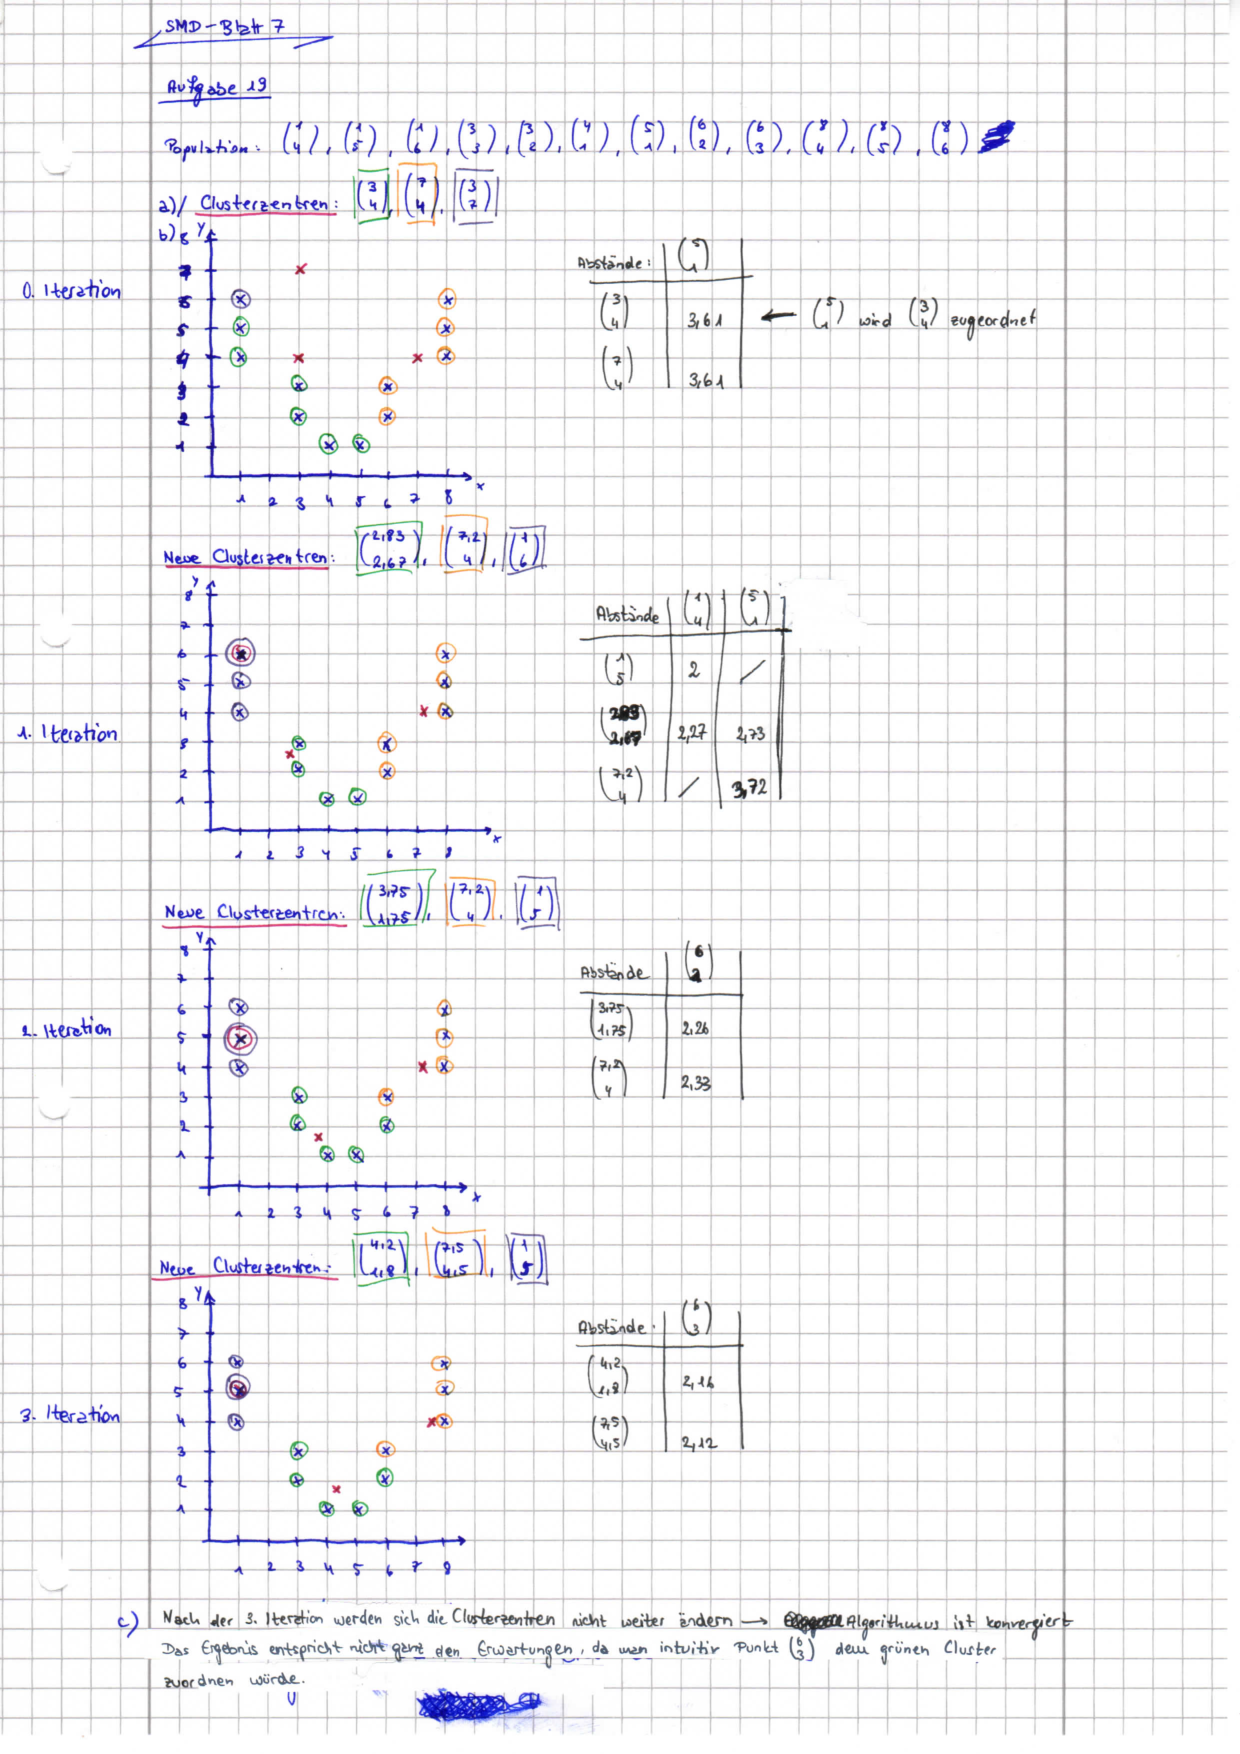
\includegraphics[scale=0.8]{Aufgabe19/SMD_Blatt07.pdf}
\end{figure}
\FloatBarrier
\paragraph{Aufgabe 20}
\subparagraph{a)}
Die Lossfunktion ist ein Ma\ss für die Ungenauigkeit zwischen einem vorhergesagten Wert $\hat{y}$ und einem richtigen Wert $y$.
Eine gebräuchliche Kostenfunktion ist in etwa die Kreuzentropie
\begin{equation}
  H(p, q)=-\sum_k p(k) \log{q(k)} \label{eq:H}
\end{equation}
\begin{center}
 \tiny {($ p(x) \: \hat{=} \:\text{wahre Wahrscheinlichkeitsdichte}$, $ q(x) \: \hat{=} \:\text{geschätzte Wahrscheinlichkeitsdichte}$)}
\end{center}
Die Gleichung \eqref{eq:H} liefert kleinere Werte je näher $p$ und $q$ sind.

\subparagraph{b)}
Die Lossfunktion kann minimiert werden, indem man der Richtung des Gradienten in jedem Schritt folgt.

\subparagraph{c)}
Aktivierungsfunktionen haben die Funktion, die Anregung einer Zelle im Zellkern zu simulieren und somit die Ausgabefunktion des Neurons zu bestimmen.
3 gängige Aktivierungsfunktionen sind:
\begin{enumerate}
  \item sigmoid-Funktion:$\sigma(x)=\frac{1}{1+\exp{-x}}$
  \item Tangens hyperbolicus :$\tanh(x)$
  \item Rectified Linear Unit: $max(0, x)$
\end{enumerate}

\subparagraph{d)}
Ein Neuron bildet die Basis eines neuronalen Netzwerkes und ist einem Neuron in der Biologie nachempfunden. Mit den zugeweisenden Eingaben $x_i$ und Gewichte $W_i$ wird die
Ausgabefunktion
\begin{equation}
  \text{net}_j=\sum_{i=0}^{n} x_i w_{ij}
\end{equation}
definiert.
Die Aktivierung dagegen ist definiert durch
\begin{equation}
  o_j=\phi(\text{net}_j-\theta_j)
\end{equation}
\begin{center}
 \tiny {($ \phi \: \hat{=} \:\text{Aktivierungsfunktion}$, $ \theta \: \hat{=} \:\text{'Schellenwert' zur Verschiebung der Gewichtung}$)}
\end{center}

\subparagraph{e)}
Anwendungsbeispiele sind zum Beispiel:
\begin{enumerate}
  \item Gesichts/Bilderkennung
  \item Texterkennung
  \item Spracherkennung
\end{enumerate}
Diese Beispiele eignen sich besonders, da kein (oder wenig)  explizites Wissen vorhanden sein muss, um diese zu identifizieren.
